\chapter{Model}
In this chapter, we present our preprocessing steps and the incremental approach used to determine our final multimodal architecture. We conduct experiments with each model to demonstrate that the combined features enhance the accuracy of our final regression model.

\section{Preliminary}
Before starting the training process, we ensured our data was prepared and optimized for learning. This section details the preprocessing steps, data splitting strategy, and the metrics used throughout our model development.

\subsection{Preprocessing}
To enhance the learning process, we normalized our values using various tools from \textit{scikit-learn} \cite{scikit-learn} and \textit{pickle} \cite{pickle}. Scikit-learn, a Python module, offers valuable functions and classes for such tasks. We used pickle to save the fitted encoders and preprocessors for future inference.

We began by converting the boolean columns to integer values, followed by encoding the categorical columns. Initially, we attempted one-hot encoding for the categorical columns. One-hot encoding transforms each possible entry in the categorical columns into its own column with boolean values. However, this approach was suboptimal because our model's features became extremely sparse, with each manufacturer having five to thirty models. Instead, we opted for target encoding, which calculates the mean of the target variable where the encoded value is present.

Next, we normalized our values, which were now entirely numerical. Due to the differences in magnitude caused by our target encoding approach, it was crucial to use StandardScaler from scikit-learn to normalize the input values. StandardScaler calculates the mean and standard deviation for each feature, subtracts the mean from the current value, and divides the result by the standard deviation.

An unconventional experiment that proved beneficial for our task was scaling our target variable, the price. Although scaling the target variable is unusual in regression models, this approach improved the accuracy across all our models. We make sure to save the fitted scaler for future use, as we need the unscaled predictions for our users.

Descriptions do not require additional preprocessing, thanks to the formatting techniques applied during our formatting, cleaning, and analysis processes. These techniques, discussed earlier in the thesis, will be replicated during inference to ensure accurate results. The use of the tokenizer is detailed in \hyperref[sec:bert]{Section 4.3}. 

For training our FastVit model, we use its predefined preprocessing function with the \textit{is\_training} attribute set to \textit{True}. This function employs various traditional techniques, such as flipping, rotating and zooming, while also resizing the images to the model's required size of 256x256 pixels. This preprocessing step allows for a better generalization of the image encoder, making it more robust to the variety that we expect from user input. At inference, we are setting the attribute to \textit{False}, letting the predefined function do all the required preprocessing steps.

\subsection{Splitting Strategy}
In order for our experiments to be comparable, we adopted a pre-splitting strategy. Our splitting strategy and some preprocessing steps take place only one time, for all our experiments, therefore assuring that the results are comparable.

In our sparse dataset, it was crucial to distribute the data as evenly as possible. The distribution needed to match not only in terms of target value but also the features fed into the model. We aimed to avoid situations where a manufacturer, model, or other key features appeared only in one of the datasets. Initially, we attempted a clustering method using k-means, but after analyzing the distribution between our train and test datasets, we found it did not provide accurate separation.

Our final and most effective method was using a stratify key generated from multiple categorical columns:

\begin{lstlisting}
stratify_columns = ["manufacturer", "model", "fuel", "chassis", "is_automatic", "sold_by_company"]

for train_index, test_index in sss.split(df, df["stratify_key"]):
    train_set = df.iloc[train_index]
    test_set = df.iloc[test_index]
\end{lstlisting}

This approach resulted in a well-balanced split between the train and test datasets, as evidenced by the nearly identical distribution by price plot, scaled to the number of samples presented in \hyperref[fig:data-split]{Figure 4.1}. We used 80\% of our data for training and 20\% for testing.

\begin{figure}[ht]
    \centering
    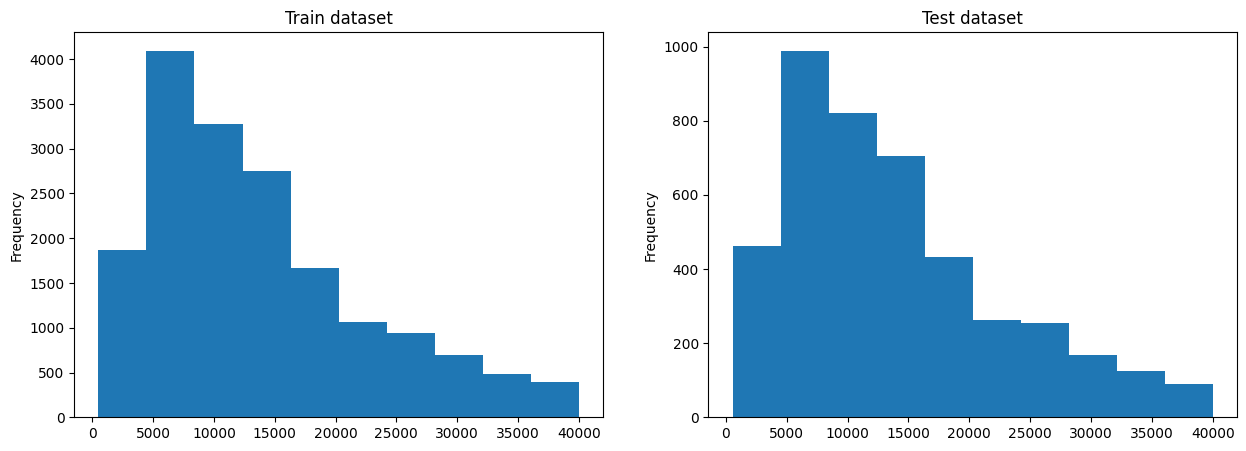
\includegraphics[width=\linewidth]{images/priceprediction/model/data_split.png}
    \caption{Train Test Data Split}
    \label{fig:data-split}
\end{figure}

\subsection{Metrics}

In this section, we describe three important metrics that we have used for evaluating our regression models: Mean Absolute Error (MAE), Mean Squared Error (MSE), and R-squared (\(R^2\)).

\subsubsection{Mean Absolute Error (MAE)}
\[ \text{MAE} = \frac{1}{n} \sum_{i=1}^{n} |y_i - \hat{y}_i| \]

\textbf{MAE}, also usually referred to as L1Loss, measures the average over the sum of absolute differences between the ground truth and predicted value

\textbf{Interpretation:}
\begin{itemize}
    \item A lower MAE indicates a better fit.
    \item MAE is less sensitive to outliers since it doesn't square the error compared to MSE, but it doesn't highlight large errors as much as MSE does.
\end{itemize}

\subsubsection{Mean Squared Error (MSE)}
\[ \text{MSE} = \frac{1}{n} \sum_{i=1}^{n} (y_i - \hat{y}_i)^2 \]

\textbf{MSE} also usually referred to as L2Loss, measures the average over the sum of the squared differences between the ground truth and predicted values.

\textbf{Interpretation:}
\begin{itemize}
    \item A lower MSE indicates a better fit.
    \item MSE gives a higher weight to large errors, thus being sensitive to outliers and penalizing them more than MAE.
\end{itemize}

\subsubsection{R-squared (\(R^2\))}
\[ R^2 = 1 - \frac{\sum_{i=1}^{n} (y_i - \hat{y}_i)^2}{\sum_{i=1}^{n} (y_i - \bar{y})^2} \]

\textbf{\(R^2\)} or \textit{coefficient of determination} provides valuable insights into how well the data fits the regression model. 

\textbf{Interpretation:}
\begin{itemize}
    \item \( R^2 \) ranges from 0 to 1, but sometimes can be even negative.
    \item A high \(R^2\) value means that the model explains the data it gets in a big proportion, meaning the data is representative for the task we are pursuing.
    \item A low \(R^2\) suggests that the data has more noise and less relevance to the model.
    \item Negative \( R^2 \) values can occur if the model performs worse than simply predicting the mean of the observed data.
\end{itemize}

\subsubsection{Summary}

These metrics together provide a comprehensive understanding of model performance from different perspectives.

\section{MLP - Structured Data}
Working with our self-scraped dataset, we lacked a baseline performance score. Our initial experiment involved creating a multilayer perceptron (MLP) as our baseline.

We utilized \textit{PyTorch} \cite{pytorch} as our deep learning framework. PyTorch simplifies the development of deep learning models by providing an accessible abstraction layer over the complex mathematical operations required. One of its key features is the utilization of CUDA (Compute Unified Device Architecture) cores for GPU acceleration, which significantly improves both training and inference computations. While \textit{TensorFlow} \cite{tensorflow} is a common alternative, we chose PyTorch due to its ease of use and support across all platforms, ensuring our code's reproducibility on various operating systems. In contrast, TensorFlow has support for CUDA only on Linux machines, which could limit its applicability.

The architecture of the Multilayer Perceptron (MLP) that yielded the best results after extensive fine-tuning comprises two fully connected (linear) hidden layers. The first hidden layer contains 128 neurons, while the second one contains 64 neurons.

ReLU activation functions are applied to each hidden layer to introduce non-linearity. Additionally, we use dropout with a rate of 0.2 on the second hidden layer to help prevent overfitting during the training phase.

For training this model, we will use the Adam optimization function with a learning rate of 1e-4 (0.0001). 

We use the L1Loss function as our loss metric. We chose L1Loss over the more commonly used L2Loss for regression tasks because our self-scraped dataset still contains some outliers that we do not want to unduly influence our model. This issue with outliers is evident in our final results presented in \hyperref[tab:best-results]{Table 4.1}, where the R-squared score is high, but the performance is not optimal.

During our training phase, we also implemented two important techniques: reducing the learning rate on a plateau and early stopping. Reducing the learning rate helps us to adjust the learning process when progress stalls, thereby improving convergence, and also allowing our model to focus on details later in the training session. Early stopping allows us to halt the training session early if overfitting or lack of further learning is detected, ensuring we save the best model from each training session.

\section{BERT - Text Encoder}
\label{sec:bert}
\textbf{B}idirectional \textbf{E}ncoder \textbf{R}epresentation from \textbf{T}ransformers (BERT) \cite{bert} is a transformer-based architecture, designed for encoding continuous pieces of text data. BERT builds on the transformer model introduced in the paper \textit{"Attention is All You Need"} \cite{attention}, which details the architecture's encoding and decoding components. BERT consists of multiple transformer encoder layers stacked on top of each other, similar to how GPT (Generative Pre-trained Transformer) is composed of stacked decoder layers. Its key features include faster processing speed, the ability to process multiple words simultaneously, and a deep understanding of context in a bidirectional manner.

For our problem, which involves inputs in Romanian, we will use a pre-trained version of BERT Base called Romanian BERT, introduced in the paper \textit{"The Birth of Romanian BERT"} \cite{dumitrescu-etal-2020-birth}. This model, based on BERT Base, contains 110 million trainable parameters and has been pre-trained on a 15GB corpus of Romanian text data.

Initially, we considered training a base BERT model from scratch. This idea stemmed from the unique language structure of our advertisement descriptions, which often contain numerous enumerations. However, we quickly realized that our data was insufficient for this approach, so we opted to use the pre-trained Romanian BERT model.

Throughout our training phase and during inference, we utilize the pre-trained tokenizer provided with the Romanian BERT model. The arguments passed to the tokenizer remain consistent. Although our data is already uncased, we add an extra layer of precaution by setting the \textit{do\_lower\_case} argument to \textit{True}. We instruct the tokenizer to add special tokens because we are particularly interested in the [CLS] token. Additionally, we set the maximum length accepted by BERT to 512, with both padding and truncation enabled. This maximum length is chosen because, after analyzing our descriptions, we found they often exceed this length, making truncation necessary.

\begin{lstlisting}
tokenizer = AutoTokenizer.from_pretrained("dumitrescustefan/bert-base-romanian-uncased-v1", do_lower_case=True, add_special_tokens=True, max_length=512, padding=True, truncation=True)
\end{lstlisting}

The fine-tuning phase of BERT involves two stages. The first stage trains BERT to understand the language, while the second stage fine-tunes it for our specific task, which is regression.

To train BERT to understand the language, we employed a self-supervised method known as masked language modeling (MLM). In this approach, 15\% of the tokens are masked, and BERT's task is to predict these missing words. For task-specific fine-tuning, we added two additional layers after the BERT embeddings. The first is a fully connected layer with 768 neurons, followed by a second layer with a single neuron representing our output. We use the [CLS] token embedding from BERT as the input to the first newly introduced layer, leveraging its comprehensive representation of the entire input.

\section{FastVit - Image Encoder}
FastVit \cite{fastvit} is a hybrid vision transformer architecture optimized for speed while maintaining high performance. It combines the strengths of both Vision Transformers (ViTs) and Convolutional Neural Networks (CNNs) to overcome their individual limitations. By integrating CNNs, FastVit enhances overall computation speed and improves local feature extraction and pattern recognition. The inclusion of Vision Transformers addresses the primary 
limitation of CNNs, which excel at finding fixed spatial relationships. By leveraging the attention mechanism from vision transformers, FastVit can understand the global context and capture relationships between different parts of an image.

For our task, we are using a pre-trained version of FastVit T8 for the same reason as with BERT: the lack of sufficient data. This pre-trained model has been trained on the IMAGENET1K dataset. We fine-tune the model for our regression task by adding the same layers as in our BERT approach. We also utilize the [CLS] token as the input to our newly introduced layers, utilizing its comprehensive representation.

\section{Multimodal Architecture}
Our final and best architecture for our multimodal model, showcased in \hyperref[fig:model-architecture]{Figure 4.2}, comprises fine-tuned versions of both BERT and FastVit, serving as text and image encoders, respectively. We utilize these models without the added fully connected layers, focusing on their pre-trained feature extraction capabilities for our regression task.

By using these fine-tuned encoders, we use their ability to extract essential features, which we then concatenate with our structured data, resulting in an input of 1546 features. In this setup, all layers of our encoders are frozen. However, a potential future enhancement could involve unfreezing these layers to enable full end-to-end fine-tuning throughout our architecture.

The concatenated input is then passed through the Multilayer Perceptron (MLP) shown in \autoref{lst:multimodal}, on which we apply ReLU activation functions and Dropout to introduce non-linearity and prevent overfitting, respectively. Additionally, early stopping is used to halt training if overfitting is detected or if there is no further improvement.

\begin{lstlisting}[label={lst:multimodal}]
model = nn.Sequential(
    nn.Linear(1546, 128),
    nn.ReLU(),
    nn.Dropout(0.2),
    nn.Linear(128, 64),
    nn.ReLU(),
    nn.Dropout(0.2),
    nn.Linear(64, 1)
)
\end{lstlisting}


\begin{figure}[ht]
    \centering
    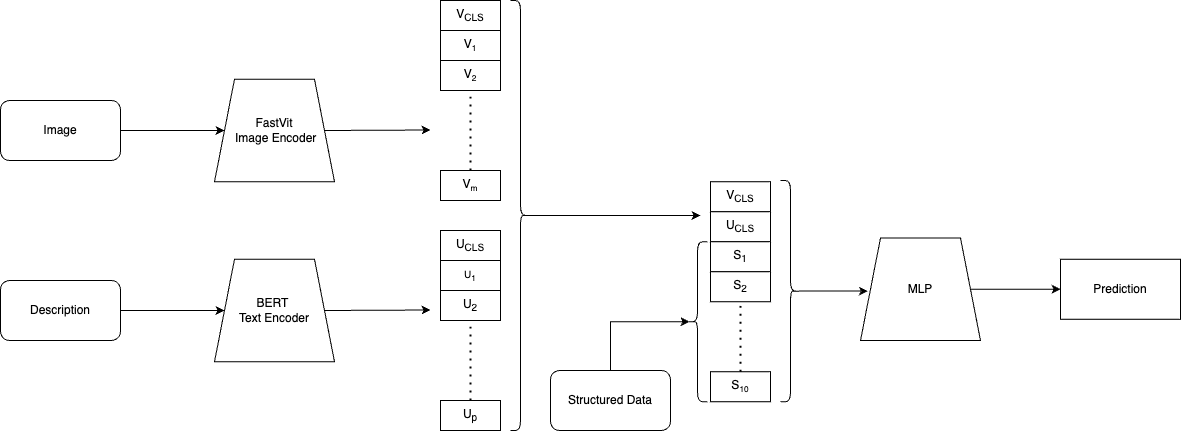
\includegraphics[width=\linewidth]{images/priceprediction/model/arch.png}
    \caption{Multi-modal architecture}
    \label{fig:model-architecture}
\end{figure}

In \hyperref[fig:multimodal-results]{Figure 4.3}, we present the training plots for our best multimodal model training session. The plots demonstrate a stable learning process. Notably, our test dataset initially performs better than the training set until epoch 130, where their performance converges. This suggests that the test dataset might be easier to predict, but given the small difference, we did not pursue further adjustments.

\begin{figure}[ht]
    \begin{subfigure}[b]{0.48\linewidth}
        \centering
        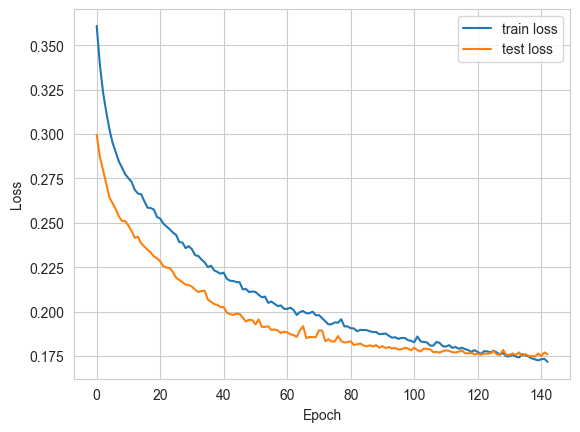
\includegraphics[width=\linewidth]{images/priceprediction/results/multimodal_loss.png}
        \caption{Loss (MAE)}
        \label{fig:multimodal-loss}
    \end{subfigure}
    \hfill
    \begin{subfigure}[b]{0.48\linewidth}
        \centering
        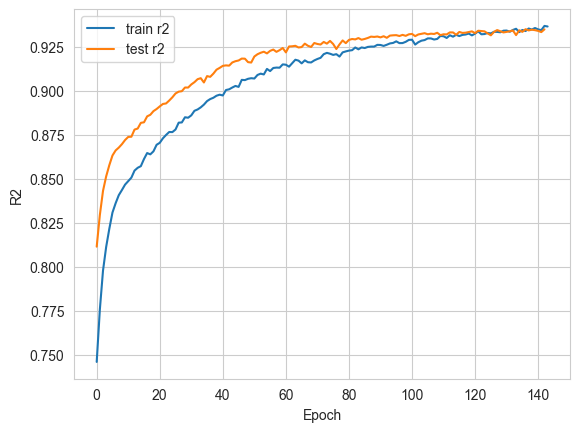
\includegraphics[width=\linewidth]{images/priceprediction/results/multimodal_r2.png}
        \caption{\(R^2\)}
        \label{fig:multimodal-r2}
    \end{subfigure}
    \caption{Multi-modal Training Plots}
    \label{fig:multimodal-results}
\end{figure}

\section{Results analysis}
In \hyperref[tab:best-results]{Table 4.1}, we present the results of our regression models, including both individual model outcomes and the final multimodal architecture. The results demonstrate that the most valuable features are found in the structured data, followed by descriptions and images. The best performance is observed in the multimodal architecture, validating our hypothesis that descriptions and images of advertisements provide valuable information for improving predictive accuracy.

\begin{table}[ht]
\centering
\begin{tabular}{lcccc}
    \textbf{Model} & \textbf{Environment} & \textbf{MAE} & \textbf{R2} \\ \hline
    \multirow{2}{*}{MLP} & Train & 1650 & 0.90 \\
                         & Test & 1698 & 0.895 \\ \hline
    \multirow{2}{*}{FastVit} & Train & 4007 & 0.623 \\
                             & Test & 4051 & 0.618 \\ \hline
    \multirow{2}{*}{BERT} & Train & 2427 & 0.85 \\
                          & Test & 2655 & 0.80 \\ \hline
    \multirow{2}{*}{Multimodal} & Train & \textbf{1522} & \textbf{0.936} \\
                                & Test & \textbf{1561} & \textbf{0.934} \\
\end{tabular}
\caption{Models best results}
\label{tab:best-results}
\end{table}
